\chapter{Überblick}

\section{Idee}

In der modernen, vernetzten Gesellschaft nimmt die Akzeptanz für Dienste und Lösungen, die über das Internet bereitgestellt werden, zu. On-Demand-Services, vor allem im Bereich Musik und Filme, zählen hier zu den wichtigsten und komfortabelsten Lösungen, um dem Konsumenten jederzeit das gewünschte Produkt liefern zu können. Auch im Softwarebereich nimmt die Bedeutung von sofort herunterladbaren Produkten zu. So bietet ein großer Versandhändler mittlerweile bei manchen Softwareprodukten Downloadversionen an und auch große wie kleine Softwarehersteller bieten eine Downloadvariante ihrer Programme über die eigene Website an. Jedoch ergibt sich daraus eine für den Kunden unüberschaubare Fragmentierung in der Anbieterlandschaft. Woher soll ein Kunde nach längerer Zeit z.B. im Falle einer notwendigen Neuinstallation wissen, ob er die Lizenz eines Programmes über die Herstellerwebsite oder einem Händler erworben hat? Woher kann er das Programm runterladen um seine Lizenz wieder zu benutzen?

Hier setzt unsere Geschäftsidee an: ein All-In-One-Lösung für Softwarelizenzen. Es geht hierbei um die Entwicklung einer Plattform, die Kunden und Anbieter von Programmen auf einfache Art und Weise zusammen bringt. Die Plattform umfasst einen Client für Windows, Linux und Mac, in welchem die Lizenzen eines Benutzers verwaltet werden. Der Benutzer kann hier gekaufte Programme jederzeit mit einem Klick herunterladen und installieren. Wie schon erwähnt richtet sich die Plattform an die drei Betriebssysteme Windows, Linux und Mac, bietet also eine größtmögliche Reichweite in Bezug auf x86-Systeme. Der Client greift direkt auf ein Shopsystem zu, welches auch über eine Website erreicht werden kann. Hier kann im Katalog geblättert werden und neue Software gekauft werden. Im Spielesoftwarebereich gibt es bereits eine Lösung, die sich großer Beliebtheit erfreut: Steam. Hiermit lässt sich die Plattform „Softladen“ am besten vergleichen. Wie Steam soll auch die „Softladen“-Plattform verschiedene Funktionen bzw. Services unterstützen. Benutzerdaten eines angebotenen Programms, z.B. Einstellungen und mit dem Programm erstellte Dokumente, sollen synchronisiert werden können. Um den Kunden große Freiheit zu gewähren soll dies optional sein. Denkbar wäre, jedem Kunden ein bestimmtes Kontingent an Cloudspeicher für die erstellten Dateien zu gewähren. In Zeiten von billig verfügbaren Cloudspeicher wäre aber auch eine grenzenlose Speicherung denkbar, denn die Dateien müssen über die vom Client verwalteten Programme erstellt werden, was eine natürliche Limitierung darstellt. 
Eine weitere Funktion ist, wie schon erwähnt, die Crossplattformtauglichkeit. Das heißt, wenn ein Benutzer den Client z.B. unter Windows benutzt, sich ein Programm kauft, später zu Linux wechselt und das Programm ist dafür verfügbar, dann kann er es einfach dafür runterladen.
Damit die Plattform auch für Hersteller von Software interessant ist, kann der Client auch als eine Art Kopierschutz fungieren. Jede Lizenz ist mit dem Konto eines Benutzers verknüpft und kann nur gestartet werden, wenn der Benutzer im Client angemeldet ist. Der Benutzer kann den Client auf unendlich vielen verschiedenen Rechnern installieren, jedoch darf nur einer der Rechner bei Softladen angemeldet sein, was eine parallele Mehrfachbenutzung eines Accounts verhindert. Natürlich kann ein Benutzer nicht immer online sein, weshalb auch die Implementierung eines Offline-Modus notwendig ist. Es ist außerdem möglich, dass die Hersteller ihre Software in Abo-Modellen anbieten. Diese Art der Softwaredistribution ist aktuell im kommen (Beispielsweise hat Adobe vor, ihre Produkte darauf auszurichten, Microsoft benutzt das bei Office 360 bereits). Diese Abos können einfach über die Plattform verwaltet werden.
Attraktiv für die Hersteller zu sein ist sehr wichtig, denn diese müssen für ein Mitwirken erst einmal gewonnen werden. 
Nur wenn eine kritische Masse an Programmen im Shop verfügbar ist, ist die Plattform auch für Benutzer attraktiv. Um diese Attraktivität zu erhöhen ist die Implementierung einer „Sales“-Funktion angedacht. Hiermit soll es möglich sein, Software, in Absprache mit dem Hersteller, vergünstigt für einen bestimmten Zeitraum anzubieten. Normalerweise gibt es kaum Vergünstigungen bei (Desktop-) Software. Diese sind aber sehr hilfreich, um Kunden zum Kauf zu animieren, auch wenn sie das Programm vielleicht nicht unbedingt brauchen. Damit erreicht man eine erhöhte Kundschaft. Damit dem Kunden das Kaufen so angenehm wie möglich gemacht wird, soll eine Vielzahl von Bezahlsystemen integriert werden. Als Beispiele seien Paypal, Kreditkarte, Amazon Checkout und giropay genannt.
Besonders für kleinere Entwickler bietet eine solche Softwareplattform Vorteile. Erstens wird eine viel höhere Kundschaft erreicht, denn ein Empfehlungssystem lässt sich einfach in dem Shop implementieren. Zweitens bietet die Plattform die Übernahme des Vertriebes, ggf. muss der Entwickler keine eigene Infrastruktur aufbauen. Damit sichergestellt wird, dass Programme in das System kommen, die eine gewisse Qualität bieten und vor allem nicht schädlich sind, ist eine Qualitätssicherungsprüfung von Programmen von unbekannten Herstellern notwendig. Diese könnte extern geschehen oder wird von Softladen angeboten. Auch das ist ein Vorteil für kleine oder unbekannte Entwickler, denn diese können dann ihr Programm mit einer Art Zertifizierung bewerben.
				
\section{Zeitplan}

Bis zum operativen Start des Unternehmens, also dem Zeitpunkt, an dem die oben genannten Dienstleistungen erbracht werden können, befindet sich das Unternehmen in der Strukturierungs- und Entwicklungsphase. Abb. 1 zeigt den zeitlichen Ablauf dieser  Phase.

%\begin{figure}[h]
%         \centering
%                 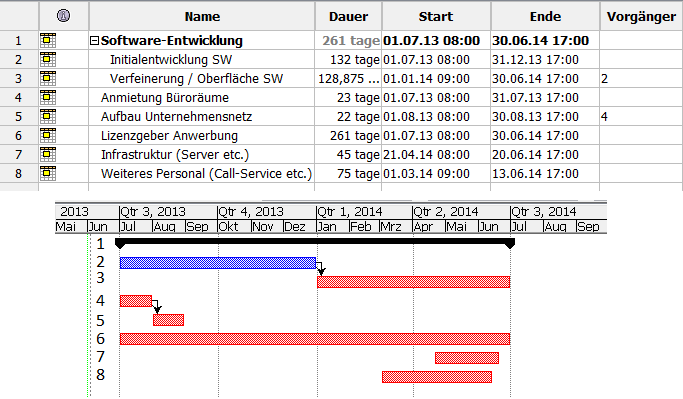
\includegraphics[scale=1.00]{zeitplan.png}
%                 \caption{Zeitplan}
%         \label{fig:NM}
% \end{figure}

Der veranschlagte Zeitraum für diese Phase entspricht exakt einem Jahr. Er ist unterteilt in

\begin{itemize}
	\item Entwicklung der Software
	\item Infrastruktur (Firma, Ressourcen)
	\item Infrastruktur (Verträge mit Lizenzgebern)
	\item Personalmanagement
\end{itemize}

Die Entwicklung der Software ist grob unterteilt und beschäftigt sich in den ersten beiden Quartalen mit der Basis des Klienten und soll grundlegende Funktionen ermöglichen. Diese werden den Erwerb von Lizenzen, die Verwaltung dieser in Kategorien und die permanente Zugänglichkeit der Downloads umfassen. Die zweite Phase der Entwicklung wird auf Usability-Aspekte, also optimierte Oberflächen und Benutzerfreundlichkeit ausgerichtet sein. Dieser Aspekt soll natürlich auch nach dem operativen Start des Unternehmens fortgeführt werden.

Die Infrastruktur ist ebenfalls zu unterteilen. Zum einen gilt es, betriebliche Prozesse zu entwerfen und zu organisieren. Zum anderen müssen Ressourcen für den Betrieb des Unternehmens geschaffen werden, also ggf. Server, Service-Aspekte (Hotlines etc.), mögliche Bezahlsysteme (Beispiele oben genannt) und weiteres in Betracht gezogen werden. 

Für die Betreuung eines Kundenstammes in Form von Service-Leistungen, sowie für Wartung und Organisation ist eine Erweiterung des Personals geplant. Auch diese muss rechtzeitig vor Markteinstieg vollzogen sein und wird deshalb vor.

\section{Strategische Ziele}

Langfristig gilt es, unter den Online-Consulting-Unternehmen eine Spitzenposition einzunehmen. Gegenüber anderen Unternehmen dieser Art wird das Alleinstellungsmerkmal einer Client-Software den entscheidenden Ausschlag geben, um sich in zwei Bereichen zu etablieren: Einem Stamm an Vertragspartnern, der Möglichkeiten für ein reichhaltiges Angebot an Software bietet, sowie einem breiten Feld an Kunden für die gebotenen Dienstleistungen.

Mittelfristig werden sich die Ziele auf eine schnelle Reputations-Steigerung und einer damit verbundenen Marktwertsteigerung des Unternehmens beziehen. Beispielsweise soll neben Verträgen mit großen Namen der Branche eine verlässliche Plattform für kleine Entwickler geschaffen werden, die eine Verbreitung von unbekannter Software vereinfacht. Käufer haben auf diese Art eine bessere Übersicht.

Kurzfristig steht die erfolgreiche Markteinführung mit einer ausreichend großen Auswahl von Produkten im Vordergrund. Hier muss die richtige Balance bei der Verteilung (auf die Plattform Softladen.de und den jeweiligen Anbieter der Software) von Einnahmen von Anfang an stimmen, damit längerfristig ein Erfolg dieses Formats überhaupt möglich ist. 

Eine Erweiterung des Konzepts ist natürlich auch möglich und kann sich beispielsweise durch den Markt selber andeuten oder durch eine Ausweitung des Produktbereichs sowie neuen Funktionen ergeben.
